\section{Attacks, Implications, and Proposed Solutions}
\begin{itemize}
	\item transaction graph attacks
	\item passive network-layer attacks
	\item statistical attacks
\end{itemize}

\section{Attack Vectors}
Given the design of the Bitcoin system, it may seem surprising that the surface for privacy- and anonymity-targeting attacks is quite large. In fact, there is a large amount of information available to attackers that may be, and has been, exploited to carry out such attacks. Perhaps most fruitful are the \emph{transaction} and \emph{user} graphs that can be constructed via network and transaction analysis. The transaction graph is a directed graph $\mathcal{T}$ with a vertex set $V(\mathcal{T})$ containing all transactions in the Bitcoin history and edge set $E(\mathcal{T})$ containing directed edges between the source (sender) and target (recipient) for each transaction. An example transaction graph is illustrated in Figure \ref{fig:transaction-graph}. The user graph is yet another directed graph $\mathcal{U}$ with a vertex set $V(\mathcal{U})$ corresponding to physical users, or entities, partaking in the Bitcoin system and edge set $E(\mathcal{U})$ corresponding to the flow of Bitcoins or funds between two users. An example user graph is illustrated in Figure \ref{fig:user-graph}. With sufficient network analysis (i.e., eavesdropping on Bitcoin traffic in the network), one may also construct a \emph{network address} graph, which is similar to the user graph with the exception that vertices represent physical IPs instead of particular users. 

%Vu - I may switch attack on privacy with anonymity and have anonymity first.  Need to reconcile user-network graphs and transaction-network graphs with attacks on privacy and anonymity.

\begin{figure}
\begin{center}
% 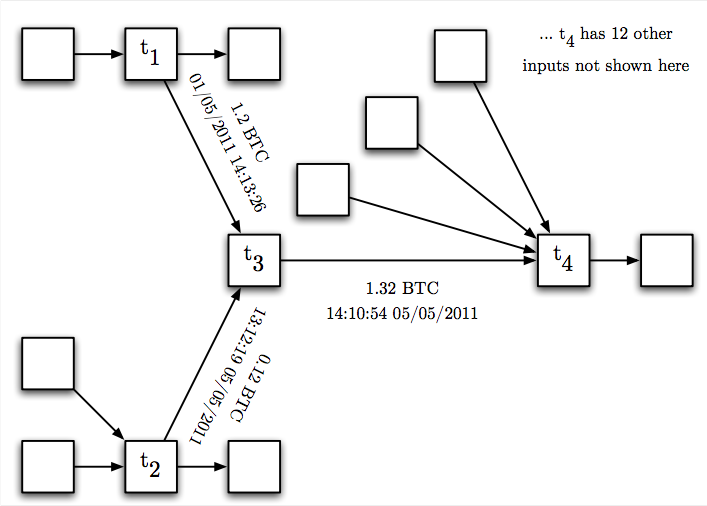
\includegraphics[scale=0.5]{images/transaction_graph.png}
\label{A sample transaction graph CITE.}
\caption{fig:transaction-graph}
\end{center}
\end{figure}

\begin{figure}
\begin{center}
% \includegraphics[scale=0.5]{images/user_graph.png}
\label{A sample user graph CITE.}
\caption{fig:user-graph}
\end{center}
\end{figure}

\subsection{Attacks on Privacy}
%Current loss of privacy through voluntary identification/off network information, flow analysis, IP tracking. Needs more info
As a currency system, Bitcoin cannot have perfect privacy. Although the information originates outside the Bitcoin network, some address ownership information are public knowledge. For instances, a store needs to have a publicly identifiable address in order to accept payment for goods or services.  Users may also disclose address ownership when asking for donations or posting on Bitcoin forums \cite{Fistful12}. Large centralized Bitcoin services such as the Mt. Gox exchange service are also able to associate users with addresses as part of their service.

The trivial attack on privacy involve using the Bitcoin block chain to follow all the transactions associated with that address. As user commonly have many addresses, a more sophisticated attack requires the adversary to link the known address with other hidden addresses and then analyze the transactions associated with those addresses. The two major heuristics for linking addresses are \emph{multi-address transactions} and \emph{shadow or change addresses}. 

Multi-address transactions are transactions with more than one source. Currently, Bitcoin allows for users to use more than one source address in a transaction, but does not allow multiple users to pay for one transaction. For example, suppose $\mathsf{addr}_A$ has 3 Bitcoins (BTC) and $\mathsf{addr}_B$ has 2 BTC. The user uses both addresses to pay 4 BTC to $\mathsf{addr}_C$ and puts the remainder of 1 BTC to $\mathsf{addr}_D$. Only one user can be the input to any transaction, therefore in this example, $\mathsf{addr}_A$ and $\mathsf{addr}_B$ belong to the same user.

\emph{Shadow addresses} or \emph{change accounts} are accounts created for change from a transaction. In the transaction above, $\mathsf{addr}_D$ is the shadow account that belongs to the same user that controls $\mathsf{addr}_A$ and $\mathsf{addr}_B$. Although not directly related to the Bitcoin system, the way Bitcoin clients handle shadow accounts can break address indistinguishability [4]. However, because shadow accounts rely on user behavior instead of an inherent property of the Bitcoin system, the shadow account heuristic is not as robust \cite{Fistful12}.

Using these two heuristics, researchers have been able cluster addresses with a common owner in a user graph where every node is a user and every edge is a transaction \cite{Shamir13-bitcoingraph,ReidHarrigan13,Fistful12}. In any node where the user has revealed ownership of an address, the user's privacy has been lost.

Another privacy loss channel is the TCP/IP layer. As previously mentioned, Bitcoin uses a peer-to-peer network to transmit transactions. Many services, such as Bit Faucet, will log and publish the IP address of users of the service. A more active attack would include malicious nodes scanning for Bitcoin clients listening to port TCP/8333 \cite{ReidHarrigan13} and open a direct connection. While proxy services like Tor can hide outbound connections, an inbound connection will not be obfuscated. By listening to transaction announcements over time, the client that first reports a transaction is the one that initiated it. This allows the malicious nodes to link transactions to IP addresses.

\subsection{Attacks on Anonymity}
%should we combine this with the privacy section?
%attacks on address indistinguishabiilty include multi-address transactions and shadow/change accounts
Researchers attempt to break the anonymity of Bitcoins in an attempt to study stolen Bitcoins [6][8]. In a similar manner to the attack on privacy, a user graph is created. 
%There is research between big data (the user and transaction graphs) and re-identifying people. Netflix and social networks (Broken Promise of Privacy: Responding to the Surprising Failure of Anonymization by Paul Ohm and De-anonymizing Social Networks by Arvind Narayanan and Vitaly Shmatikov).  Is this outside the scope of our paper? It's alluded that user transaction graphs can be used to identify real world identities, but no one has done it yet.

Intuitively, a successful attack on the anonymity of Bitcoin yields a mapping between Bitcoin addresses, or public keys, to their respective owners. Depending on the success criteria for such an attack, the attacker may seek to find a single mapping for a particular user or, quite oppositely, a mapping for as many users as possible. Accordingly, there has been substantial research investigating the degree to which anonymity is achieved \cite{ReidHarrigan13,BetterToBitter,Fistful12,Shamir13-bitcoingraph,Androulaki12-privacy}; proposed solutions presented in the literature are discussed in the following section.

KAMINSKY STARTED IT ALL!

Reid and Harrigan were the catalysis that started the research on Bitcoin anonymity. Using network analysis techniques on the Bitcoin transaction and user graphs

% Another highly debated topic is the anonymity of Bitcoin transactions. The fact that all transactions are tracked in a replicated ledger and that the details of the transactions are therefore accessible by any participant in the network would suggest that privacy is not possible. However, Nakamoto claims that, since the identities of the owner of an account and the identity of the account are kept separate, the privacy can be said to be pseudonymous. Reid et al. [15] analyze this claim and point out that by colluding the information of multiple accounts that participated in a transaction details about the owner can in fact be recovered. Shamir et al [17] analyzed the transaction graph, deriving some global statistics, including an estimate that 78% of the issued bitcoins are not circulating, and an in depth analysis of a highly active region in the transaction graph. Elias [8] discussed some legal, and moral, aspects of the anonymity, or lack thereof, in Bitcoin.

\subsection{Current and Proposed Solutions}
%Centralized mixes similar to Chaums anonymous email (BitFog, BitLaundry, Blockchain.info) and decentralized mixes (Zerocoin).

% The anonymity problem in Bitcoin was later addressed by ZeroCoin [13] which allows the implementation of a Zero- Knowledge based decentralized coin mixing service. Earlier Hanke et al. [10] presented a Pay-to-Contract Protocol that is built on top of Bitcoin and secures transactions between
% merchants and their clients. CommitCoin [6] is another system that builds on the blockchain to carbon date commitments.

%[5]Dorit Ron and Adi Shamir. Quantitative Analysis of the Full Bitcoin Transaction Graph. IACR Cryptology ePrint Archive 584 (2012).

%[6] Sarah Meiklejohn, Marjori Pomarole, Grant Jordan, Kirill Levchenko, Damon McCoy, Geoffrey M. Voelker, and Stefan Savage. 2013. A fistful of bitcoins: characterizing payments among men with no names. In Proceedings of the 2013 conference on Internet measurement conference(IMC '13). ACM, New York, NY, USA, 127-140

%[7] Fergal Reid and Martin Harrigan. 2013. An Analysis of Anonymity in the Bitcoin System. Security and Privacy in Social Networks. Springer, New York, NY, USA, 197-223

%[8] Dan Kaminsky. 2011. Black Ops of TCP/IP 2011. Black Hat USA 2011. http://www.slideshare.net/dakami/black-ops-of-tcpip-2011-black-hat-usa-2011

%[9] Malte Moser. 2013. Anonymity of Bitcoin Transactions: An Analysis of Mixing Services. Munster Bitcoin Conference (MBC). July 17-18, Munster, Germany